%!TEX root = ../main.tex

\chapter{Reti neurali}\label{chp:neural-networks}
% 
Il primo modello di intelligenza artificiale (\acs{AI}) risale al 1943, dove E. McCulloch e W. Pitts cercarono di modellare un neurone come una semplice funzione predefinita. In questo modello, il neurone, generava un valore in output nel caso in cui le variabili booleane di input, una volta elaborate, superavano una soglia prestabilita\,\cite{mcculloch1943logical}. Poco dopo, nel 1950, Alan Turing, pubblicò un articolo che definiva una metodologia per testare l'intelligenza di un modello\,\cite{turing2009computing}. Questo test — noto anche come \textit{imitation game} — consisteva nel valutare se una macchina potesse imitare l'intelligenza umana stabilendo così un obiettivo per il campo dell'intelligenza artificiale, termine che venne conianto per la prima volta nella conferenza di Dartmouth nel 1956.

Dopo due anni, nel 1958, lo psicologo F. Resenblatt introdusse il \textsl{percettrone} che, a differenza del modello del '43, processava input non booleani e disponeva di pesi per bilanciare l'output\,\cite{rosenblatt1958perceptron}. Anche se il percettrone sarà alla base delle reti neurali artificiali moderne, nei dieci anni successivi alla pubblicazione dell'articolo, le aspettative iniziali non vennero soddisfatte. Nel 1968 venne pubblicato un libro il quale analizzava le prestazioni del percettrone e constatava le forti limitazioni del modello, come l'impossibilità di risolvere problemi non linearmente separabili\,\cite{minsky2017perceptrons}. In seguito ad un secondo articolo del 1973, dove si evidenziavano gli scarsi risultati ottenuti in paragone con le grandi aspettative, iniziò il \textsl{Primo Inverno dell'Intelligenza Artificiale} dove fino alla metà degli anni Ottanta molte organizzazioni governative smisero di finanziare la ricerca sull'intelligenza artificiale. L'Inverno della \acs{AI} terminò nel 1985 con l'introduzione del \textit{Gradient Descent Optimization}, algoritmo che permetteva di aggiornare i pesi in modo tale da minimizzare l'errore in una rete. Un anno dopo venne introdotto l'algoritmo della \textit{back-propagation}, fondamentale per lo sviluppo di reti neurali, costituite da più livelli di neuroni, ciascuno dei quali è collegato al livello successivo\,\cite{rumelhart1986learning}.

Nonostante il grande sviluppo nella parte algoritmistica, l'hardware non era computazionalmente adeguato da supportare le richieste di calcolo delle reti neurali artificiali. Questa carenza nella potenza di calcolo portò al \textsl{Secondo Inverno dell'Intelligenza Artificiale}, periodo in cui l'interesse scientifico si spostò su modelli che richiedevano meno potenza di calcolo, come le \textit{Support Vector Machines} (\acs{SVM}) introdotte nel 1963. Il Secondo Inverno della \acs{AI} terminò a metà degli anni Novanta quando il progresso dell'hardware riuscì a soddisfare i requisiti computazionali dei modelli basati su reti neurali. Il costante sviluppo culminò nell'ultimo ventennio quando venne introdotta la \acs{GPU}, che, insieme all'aumento dei dati disponibili, accelerò notevolmente i progressi nel campo dell'\acs{AI}\,\cite{flasinski2016introduction, muthukrishnan2020brief}.

\section{Principi di base ed evoluzione}
%
Le reti neurali artificiali (\acs{ANN}) — comunemente note come reti neurali (\acs{NN}) — mirano a rappresentare un modello semplificato del cervello, trattato come una struttura composta da neuroni. Risulta quindi essenziale comprendere il funzionamento del singolo \textsl{neurone artificiale} per poi esplorare la struttura di una rete neurale, che è un insieme di neuroni artificiali, collegati tra loro secondo precisi criterio

\subsection{Neurone artificiale}
% 
Come un neurone biologico, il neurone artificiale (Figura\,\ref{fig:artificial-neuron}) riceve un numero arbitrario $n$ di segnali in \textsl{input}, che possono essere rappresentati con la notazione $x_1, x_2, \dots, x_n$. Tali valori possono essere raggruppati nel vettore di input $\mathbf{x} = \left[x_1, x_2, \dots, x_n\right]$. Per descrivere il risultato di tutti i segnali in ingresso del neurone, si introduce una funzione $g$, che generalmente è una semplice somma algebrica dei segnali di input $x_i$, con $i\in[1,\,n]$. Ogni segnale di input, prima di essere sommato viene moltiplicato per il rispettivo peso (\textit{weight}) $w_i$, con $i\in[1,\,n]$, che appartiene al vettore dei pesi $\mathbf{w} = \left[w_1, w_2, \dots, w_n \right]$. Ne consegue che il segnale in uscita, indicato con $v$, comprenderà la somma del prodotto del segnale \textit{i}-esimo ($x_i$) con il rispettivo peso \textit{i}-esimo ($w_i$):
% 
\begin{gather}
    v = g\left(\mathbf{w}, \mathbf{x}\right) = \sum_{i = 1}^n w_i\,x_i = \mathbf{w}\,\cdot\,\mathbf{x}
    \label{eq:algebric-sum}
\end{gather}
% 
\begin{figure}[!b]
    \centering
    \begin{tikzpicture}[node distance=1cm, auto]

    % inputs
    \node[draw, rectangle] (X0) {$x_0$};
    \node[below of=X0] (dots1) {$\vdots$};
    \node[draw, rectangle, below of=dots1] (Xi) {$x_i$};
    \node[below of=Xi] (dots2) {$\vdots$};
    \node[draw, rectangle, below of=dots2] (Xn) {$x_n$};
    
    % perceptron summation
    \node [draw, circle, right=2.5cm of Xi, minimum size=1.5cm] (perceptron) {\large $\displaystyle \sum$};

    % signal output v
    \node [right=0.5cm of perceptron] (output) {};

    % activation function f(v)
    \node [draw, rectangle, right=0.5cm of output] (activation) {$f(v)$};

    % final output y
    \node [right=1cm of activation] (final_output) {};

    % input arrows with weights
    \draw [->] (X0) -- node[midway, above] {} node[midway,below] {$w_0$} (perceptron);
    \draw [->] (Xi) -- node[midway, above] {} node[midway,below] {$w_i$} (perceptron);
    \draw [->] (Xn) -- node[midway, above] {} node[midway,below] {$w_n$} (perceptron);

    \draw [->] (perceptron) -- node[above] {$v$} (activation);

    \draw [->] (activation) -- node[above] {$y$} (final_output);

\end{tikzpicture}
    \caption[Rappresentazione schematica del funzionamento di un neurone artificiale.]{Rappresentazione schematica del funzionamento di un neurone artificiale. I segnali in input $x_i$ vengono moltiplicati con i rispettivi pesi $w_i$ e sommati tra loro; il risultato $v$ viene processato dalla funzione di attivazione $f(v)$ che restituisce l'output $a$.}\label{fig:artificial-neuron}
\end{figure}
% 
\noindent Per attivare un neurone, è necessario che il segnale $v$ prodotto in \textsl{output} sia superiore ad una soglia prescelta, indicata con $b$. Questo si traduce nel sottrarre tale valore al segnale $v$ e verificare che il risultato sia maggiore o minore di zero.
% 
\begin{gather*}
    \sum_{i = 1}^n w_i\,x_i \,\geq\, b
    % 
    \hspace{10px} \Rightarrow \hspace{10px}
    % 
    \sum_{i = 1}^n w_i\,x_i - b \,\geq\, 0
\end{gather*}
% 
\noindent Il valore sottratto alla somma, detto \textit{bias}, può essere inglobato nella somma algebrica. È sufficiente introdurre una componente aggiuntiva $x_0 = 1$ nel vettore di input $\mathbf{x}$ ed una componente $w_0 = -b$ nel vettore dei pesi $\mathbf{w}$. In questo modo, l'equazione\,\ref{eq:algebric-sum} può essere riscritta con l'indice $i$ che parte da 0, come segue:
% 
\begin{gather*}
    v = g\left(\mathbf{w}, \mathbf{x}\right) = \sum_{i = 0}^n w_i\,x_i = \mathbf{w}\,\cdot\,\mathbf{x}
\end{gather*}
% 
Il criterio che descrive l'attivazione del neurone artificiale è riassunto nella \textsl{funzione di attivazione}, chiamata $a = f(v)$. La funzione di attivazione più semplice che descrive tale criterio la funzione \textsl{gradino} \textbf{1}$(v)$, descritta graficamente nella Figura\,\ref{fig:step-function}:
% 
\begin{gather*}
    a(v) = \text{\textbf{1}}(v) =
    \begin{cases}
        1 \hspace{20px} \text{se } v\geq0\\
        0 \hspace{20px} \text{se } v<0
    \end{cases}
\end{gather*}
% 
\begin{figure}[!b]
    \centering
    \begin{tikzpicture}
    \begin{axis}[
        axis lines = middle,
        xlabel = $v$,
        ylabel = {\textbf{1}$(v)$},
        ymin=-0.2, ymax=1.2, % control the vertical limits
        xmin=-3, xmax=3,     % control the horizontal limits
        xtick={-2,-1,0,1,2}, % x-axis ticks
        ytick={0,1},         % y-axis ticks
        domain=-3:3,
        samples=100,
        width=10cm,
        height=6cm,
        enlargelimits
    ]
        % Plot the step function
        \addplot[
            red,
            thick,
            domain=-3:0,
        ] {0}; % Plot f(x) = 0 for x < 0

        \addplot[
            red,
            thick,
            domain=0:3,
        ] {1}; % Plot f(x) = 1 for x >= 0

        % Add a filled circle for the closed part of the step at x = 0, y = 1
        \addplot[only marks, mark=*, black] coordinates {(0, 1)};
        
        % Add an open circle for the open part of the step at x = 0, y = 0
        \addplot[only marks, mark=o, black] coordinates {(0, 0)};
        
    \end{axis}
\end{tikzpicture}
    \caption[Grafico della funzione gradino \textsl{1}$(v)$.]{Grafico della funzione gradino \textbf{1}$(v)$. Si osserva che vale zero per valori strettamente minori di zero e uno per valori maggiori o uguali a zero.}\label{fig:step-function}
\end{figure}

Analogamente alle reazioni agli stimoli esterni di un neurone biologico, anche neurone artificiale deve essere in grado di rispondere in un determinato modo quando riceve determinate informazioni. Affinchè il neurone sia capace di comporatarsi correttamente di fronte a specifici dati, è fondamentale allenarlo: è dunque necessario utilizzare un \textit{training dataset} che contenga numerosi vettori di input $\mathbf{x}$ e, per ciascuno di essi sia presente la risposta corretta che il neurone dovrebbe fornire. Lavorando con numerosi vettori di input, viene introdotta la notazione $X_j$, che indica il $j$-esimo vettore $\mathbf{x}$ del dataset. Formalmente definiamo il dataset $\mathcal{D}$ come:
% 
\begin{gather*}
    \mathcal{D} = \left\{ \left\{ X_1,\, y_1 \right\},\,\left\{ X_2,\, y_2 \right\},\,\dots\,\left\{ X_j,\, y_j \right\},\,\dots\,\left\{ X_M,\, y_M \right\} \right\}  
\end{gather*}
% 
\noindent Il dataset\footnote{Un dataset così definito è utilizzato nel \textit{supervised learning}, dove all'interno del dataset sono presenti sia i vettori in ingresso che la risposta attesa. Si contrappone l'\textit{unsupervised learning} — che non verrà trattato — dove sono presenti solo i vettori in ingresso e sono sconosciute le risposte attese.} è composto da $M$ vettori di input — $X_j$ ($j\in[1,\,M$]) — e da esattamente $M$ risposte $y_j$, che rappresentano il comportamento atteso del neurone se il vettore di ingresso è $X_j$. È quindi possibile definire la matrice $\mathbf{X}$ che contiene esattamente $M$ vettori — ciascuno in una riga — i quali sono composti esattamente da $n$ componenti (o \textit{feature}), che sono le componenti associate al vettore dei pesi $\mathbf{w}$, precedentemente introdotto. Alla matrice $\mathbf{X}$ è associato il vettore $\mathbf{y}$, anch'esso di dimensione $M$ tale per cui la componente $y_j$ sia la risposta attesa del vettore di input $X_j$.
% 
\begin{gather*}
    \begin{aligned}
        \mathbf{X} &= 
            \begin{bmatrix}
            X_1^0       & X_1^1         & \cdots     & X_1^i         & \cdots     & X_1^n     \\
            X_2^0       & X_2^1         & \cdots     & X_2^i         & \cdots     & X_2^n     \\
            \vdots      & \vdots        & \ddots     & \vdots        & \ddots     & \vdots    \\
            X_j^0       & X_j^1         & \cdots     & X_j^i         & \cdots     & X_j^n     \\
            \vdots      & \vdots        & \ddots     & \vdots        & \ddots     & \vdots    \\
            % X_{M-1}^0   & X_{M-1}^1     & \cdots     & X_{M-1}^i     & \cdots     & X_{M-1}^n \\
            X_M^0       & X_M^1         & \cdots     & X_M^i         & \cdots     & X_M^n     \\
            \end{bmatrix}
        %
        \hspace{60px}
        %
        \mathbf{y} = 
            \begin{bmatrix}
            y_1 \\ y_2 \\ \vdots \\ y_j \\ \vdots \\ y_M
            \end{bmatrix}
    \end{aligned}
\end{gather*}
% 
\noindent Da questo deriva che il vettore $X_j$ è dimensionalmente compatibile con il vettore di pesi $\mathbf{w}$ in quanto hanno esattamente la stessa dimensione.
% 
\begin{gather*}
    \begin{aligned}
        X_j = \left[ X_j^0,\, X_j^1,\,\dots,\, X_j^n \right]
        %
        \hspace{50px}
        %
        \mathbf{w} = \left[w_0,\, w_1,\, \dots,\, w_n \right]
    \end{aligned}
\end{gather*}
% 
\noindent Perciò il dataset $\mathcal{D}$ può essere riscritto attraverso la matrice $\mathbf{X}$ ed il vettore di risposte attese associato $\mathbf{y}$.
% 
\begin{gather*}
    \mathcal{D} = \left\{ \mathbf{X},\, \mathbf{y} \right\}  
\end{gather*}
% 
Con un dataset di partenza si può definire un algoritmo generico che sia in grado di descrivere il processo di apprendimento di neurone artificiale. Come descritto nell'Algoritmo\,\ref{alg:neuron-training}, dopo aver inizializzato il vettore di pesi $\mathbf{w}$, per ogni vettore $X_j$ del dataset $\mathcal{D}$, vengono calcolati il segnale $v$ e il valore della funzione di attivazione $a = f(v)$. L'idea alla base dell'algoritmo è quella di modificare il vettore di pesi $\mathbf{w}$ in funzione del risultato della funzione di attivazione rispetto al segnale processato.
% 
\begin{algorithm}[ht]
    \caption{Allenamento del neurone artificiale}\label{alg:neuron-training}
    \begin{algorithmic}
        \STATE{\textbf{Input: }Dataset $\mathcal{D}$}
        \STATE\,

        \STATE{Inizializza $\mathbf{w}$ con numeri casuali}
        \STATE$j \gets 1$
        
        \WHILE{$j \leq M$}
            \STATE\text{Calcola $v$ in funzione di $X_j$ e $\mathbf{w}$}
            \STATE\text{Determina $a$ in rapporto a $v$ e $y_j$}
            \STATE\text{Modifica $\mathbf{w}$ a seconda del risultato $a$}
            \STATE$j \gets j + 1$
        \ENDWHILE\,
    \end{algorithmic}
\end{algorithm}
% 
\noindent In questo modo, una volta processati tutti i vettori presenti nel dataset, è possibile constatare se il neurone sia stato in grado di apprendere il comportamento desiderato in funzione del vettore in ingresso\,\cite{flasinski2016introduction}.

\subsection{Modello percettrone}

Uno tra i modelli di neuroni artificiali utilizzati nelle reti neurali è il percettrone. Dato un vettore in ingresso $X_j$\footnote{Il vettore di input è indicato come la $j$-esima riga della matrice di input $\mathbf{X}$ del dataset $\mathcal{D}$.} e un vettore di pesi $\mathbf{w}$, il segnale $v$ è dato dalla somma algebrica dei prodotti di ciascuna delle componenti:
% 
\begin{gather*}
    v = g\left(\mathbf{w}, X_j\right) = \sum_{i = 0}^n w_i\,X_j^i = \mathbf{w} \, \cdot \,  X_j
\end{gather*}
% 
\noindent La funzione di attivazione $f(v)$ del percettrone è la funzione \textsl{``segno''}\,(Figura\,\ref{fig:sign-function}) — chiamata anche \textsl{gradino bipolare} — definita come segue. 
% 
\begin{figure}[!b]
    \centering
    \begin{tikzpicture}
    \begin{axis}[
        axis lines = middle,
        xlabel = $v$,
        ylabel = {\textbf{sign}$(v)$},
        ymin=-1.2, ymax=1.2, % control the vertical limits
        xmin=-3, xmax=3,     % control the horizontal limits
        xtick={-2,-1,0,1,2}, % x-axis ticks
        ytick={-1,0,1},      % y-axis ticks
        domain=-3:3,
        samples=100,
        width=10cm,
        height=6cm,
        enlargelimits,
        yticklabel style={yshift=-1ex, xshift=0.75ex} % Adjust vertical position of y-tick labels
    ]
        % Plot the step function
        \addplot[
            red,
            thick,
            domain=-3:0,
        ] {-1}; % Plot f(x) = -1 for x < 0

        \addplot[
            red,
            thick,
            domain=0:3,
        ] {1}; % Plot f(x) = 1 for x >= 0

        % Add a filled circle for the closed part of the step at x = 0, y = 1
        \addplot[only marks, mark=*, black] coordinates {(0, 1)};
        
        % Add an open circle for the open part of the step at x = 0, y = 0
        \addplot[only marks, mark=o, black] coordinates {(0, -1)};
        
    \end{axis}
\end{tikzpicture}

    \caption[Grafico della funzione segno \textsl{sign}$(v)$.]{Grafico della funzione segno \textbf{sign}$(v)$. Si osserva che vale -1 per valori strettamente minori di zero e 1 per valori maggiori o uguali a zero.}\label{fig:sign-function}
\end{figure}
% 
\begin{gather*}
    a(v) = \text{\textbf{sign}}(v) = \text{\textbf{sign}}(\mathbf{w} \cdot X_j) =
    \begin{cases}
        1 \hspace{29px} \text{se } v\geq0\\
        -1 \hspace{20px} \text{se } v<0
    \end{cases}
\end{gather*}
% 
\noindent Il particolare più importante del percettrone è la \textit{learning rule}, ovvero il criterio secondo il quel il vettore di pesi è aggiornato a seconda della predizione del modello. Se la predizione $a_j$ rispetto al vettore $X_j$ è diversa dalla risposta attesa $y_j$, allora il vettore di pesi è modificato come segue\,\cite{nielsen2015neural, flasinski2016introduction}.
% 
\begin{gather*}
    w_i \, = \, w_i \, + \, y_j\,X_j^i
\end{gather*}

Al percettrone si aggiunge anche il \textsl{neurone sigmoideo}, che è molto simile al percettrone se non per la funzione di attivazione. Anzichè avere la funzione discontinua ``segno'', viene introdotta la funzione \textsl{sigmoide} $\sigma(v)$, che è una funzione continua e restituisce valori compresi tra zero e uno (Figura\,\ref{fig:sigmoid-function}). Questa funzione, definita di seguito, rimuove le discontinuità della funzione di attivazione del percettrone e fornisce un intervallo di valori reali, piuttosto che un risultato binario.
% 
\begin{gather*}
    \sigma(v) \, = \, \frac{1}{1 + e^{-v}} \, = \, \frac{1}{1 + e^{-\mathbf{w} \cdot X_j}}
\end{gather*}
% 
\begin{figure}[!t]
    \centering
    \begin{tikzpicture}
    \begin{axis}[
        axis lines = middle,
        xlabel = $v$,
        ylabel = {$\sigma(v)$},
        ymin=-0.1, ymax=1.1, % control the vertical limits
        xmin=-5, xmax=5,     % control the horizontal limits
        xtick={-4,-2,0,2,4}, % x-axis ticks
        ytick={0,0.5,1},     % y-axis ticks
        domain=-5:5,
        samples=100,
        width=10cm,
        height=6cm,
        enlargelimits,
        yticklabel style={yshift=-1ex, xshift=0.75ex} % Adjust vertical position of y-tick labels
    ]
        % Plot the sigmoid function
        \addplot[
            red,
            thick
        ] {1 / (1 + exp(-x))};
        
        % Add horizontal lines at y = 1 for reference
        \addplot[dashed] coordinates {(-5,1) (5,1)} node[right] {};
    \end{axis}
\end{tikzpicture}

    \caption[Grafico della funzione sigmoide $\sigma(v)$.]{Grafico della funzione sigmoide $\sigma(v)$.}\label{fig:sigmoid-function}
\end{figure}
% 
Questa importante differenza rende il neurone sigmoideo più flessibile rispetto al percettrone classico e più adatto all'utilizzo nelle reti neurali\,\cite{nielsen2015neural}.

\subsection{Gradient descent}

La learning rule introdotta nel percettrone, per quanto semplice, spesso viene sostituita dalla learning rule derivante dal \textit{Gradient Descent} (\acs{GD}, rappresentato nella Figura\,\ref{fig:gradient-descent}), un approccio che mira a trovare il minimo di una funzione differenziabile, spesso chiamata funzione ``costo''. Fornito il vettore di pesi $\mathbf{w} = \left[w_0, w_1, \dots, w_n \right]$, durante l'allenamento del neurone, l'algoritmo cerca di modificare tale vettore minimizzando sempre di più l'errore tra il valore predetto dal modello e il risultato atteso. Più precisamente, data una funzione di costo $C(w)$ — detta anche \textit{loss function} — la learning rule del \acs{GD} vale:
% 
\begin{gather*}
    \mathbf{w} = \mathbf{w} - \eta\,\nabla C\left(\mathbf{w}\right)
\end{gather*}
% 
\begin{figure}[!b]
    \centering
    \input{assets/TikZ/gradient-descent.tex}
    \caption[Il gradient descent in una funzione bidimensionale.]{Il gradient descent in una funzione bidimensionale. Si osserva che l'algoritmo, attraverso il gradiente della funzione, riesce a spostarsi verso il minimo (locale o assoluto) della funzione, come una biglia di vetro.}\label{fig:gradient-descent}
\end{figure}
% 
\noindent Dove $\eta$ è un parametro positivo, chiamato \textit{learning rate} e serve per bilanciare la rapidità con cui il vettore dei pesi sia aggiornato durante l'esecuzione dell'algoritmo. Il termine $\nabla C\left(\mathbf{w}\right)$ è invece il gradiente della loss function. Il gradiente di una funzione a più dimensioni è un vettore che indica la direzione di massima crescita del valore della funzione; conseguentemente la direzione opposta è quella da seguire per raggiungere il minimo (locale o assoluto) della funzione. La Figura\,\ref{fig:gradient-descent} mostra graficamente come l'approccio \acs{GD} cerchi di raggiungere tale valore ad ogni iterazione. Si osserva che in questo caso la funzione è rappresentata in due dimensioni ma in generale la loss function è $n$-dimensionale. Questa funzione può essere una qualsiasi funzione errore: una tra le più comuni è la funzione che calcola la media del quadrato degli errori (in gergo chiamata \acs{MSE}, \textit{Mean Squared Errors}). Per fare un esempio pratico, avendo il vettore di pesi $\mathbf{w}$, un dataset $\mathcal{D}$ — definito come in precedenza — ed una funzione di attivazione $a$, la \acs{MSE} è definita come:
% 
\begin{gather*}
    C(\mathbf{w}) = \frac{1}{M}\,\sum_{j = 1}^M\,{\left[ y_j - a(\mathbf{w},\,X_j) \right]}^2
\end{gather*}
% 
\noindent L'approccio adottato da questo algoritmo, per quanto efficacie non è completamente efficiente. La complessità computazionale richiesta è notevole: ad ogni iterazione dell'allentamento del neurone, è necessario trovare il valore della derivata della loss function, che si traduce nel computare la predizione di tutti i vettori di input $X_j$ del dataset $\mathcal{D}$ e compararli con la risposta attesa $y_j$. Questo approccio, per dataset di dimensioni medio-grandi è molto poco efficiente, per quanto preciso. Inoltre è possibile che la discesa del gradiente conduca l'aggiornamento del vettore di pesi in un minimo locale della funzione errore, giungendo quindi ad una soluzione sub-ottima. Questi problemi possono entrambi essere gestiti da una variante di questo algoritmo, chiamata \textit{Stochastic Gradient Descent} (\acs{SGD}). Per ogni iterazione dell'algoritmo di allenamento, vengono presi un numero $m < M$ di vettori di input con le rispettive risposte attese e aggiornato il vettore $\mathbf{w}$ in base a questo sotto insieme del dataset, chiamato anche $mini-batch$. In questo modo la complessità computazionale viene drasticamente diminuita in quanto calcolare la derivata della loss function per una frazione ridotta del dataset richiede meno risorse. In aggiunta la casualità della scelta del mini-batch può evitare la convergenza in un minimo locale poiché rende la discesa lungo la funzione di errore leggermente più imprevedibile, diminuendo la possibilità di risultati sub-ottimi\,\cite{lu2022gradient, andrychowicz2016learning, nielsen2015neural}.

\subsection{Rete neurale}

Una rete neurale è una struttura composta da neuroni artificiali i quali sono organizzati in livelli (\textit{layers}). In una rete neurale multilivello, è sempre presente un input layer e un output layer. I livelli che si trovano tra questi sono detti livelli nascosti — \textit{hidden} layers. I neuroni dello stesso livello non sono mai collegati tra loro ma solo con i neuroni del livello precedente e del livello successivo.
% 
\begin{figure}[!b]
    \centering
    % see this link
% https://tikz.net/neural_networks/

    \caption[Rete neurale multilivello.]{Rete neurale multilivello. (immagine adattata da\,\cite{izaak2022neural}).}\label{fig:neural-network}
\end{figure}
% 
Più precisamente, data una rete neurale, i neuroni del livello $\ell$ ricevono il segnale dai neuroni del livello $\ell-1$ e, dopo aver elaborato le informazioni, inviano il segnale processato ai neuroni del livello $\ell+1$: si dice che la rete è di tipo \textit{feedforward} in quanto non sono presenti cicli nella struttura. Osservando la Figura\,\ref{fig:neural-network} si introduce una nuova notazione per i neuroni all'interno di una rete. Si definisce con $N^{(\ell)}_j$ il neurone $j$-esimo che si trova nel livello $\ell$ e si identifica con la notazione $a^{(\ell)}_j$ l'output della funzione di attivazione del neurone $N^{(\ell)}_j$. Il peso $w^{(\ell)}_{j\,,i}$ è il peso che collega il neurone $N^{(\ell - 1)}_i$ al neurone $N^{(\ell)}_j$, ovvero il collegamento tra il neurone alla posizione $i$ del livello precedente $\ell-1$ e il neurone $N^{(\ell)}_j$. Inoltre, per ogni neurone vengono esplicitati i bias: $b^{(\ell)}_j$ indica il bias associato al $j$-esimo neurone nel livello $\ell$. Presupponendo l'utilizzo di neuroni sigmoidei all'interno della \acs{NN} l'output $a^{(\ell)}_j$ del neurone $N^{(\ell)}_j$, ovvero l'output della funzione di attivazione del neurone può essere calcolato come segue: 
% 
\begin{gather*}
     a^{(\ell)}_j = \sigma\left( v \right) = \sigma\left( \sum_i w^{(\ell)}_{j\,,i} \,\, a^{(\ell - 1)}_i + b^{(\ell)}_j \right)
\end{gather*}

\noindent Questa formula indica che l'output della funzione di attivazione del neurone $N^{(\ell)}_j$ è dato dalla sigmoide calcolata sull'input del neurone. L'input è dato dalla somma algebrica degli output dei neuroni del livello precedente ($\ell - 1$), moltiplicati per i rispettivi pesi e sommati al bias del neurone. Questa notazione può essere riscritta in forma matriciale per renderla più elegante. Si definisce la matrice $\mathbf{W}^{(\ell)}$ che contiene i pesi che collegano i neuroni del livello $\ell-1$ al livello $\ell$. Allo stesso modo, si può definire il vettore $\mathbf{b}^{(\ell)}$, che contiene i bias dei neuroni nel livello $\ell$. Infine il vettore $\mathbf{a}^{(\ell)}$ contiene i valori di output delle funzioni di attivazione di tutti i neuroni al livello $\ell$. La formula può quindi essere riscritta come segue:
% 
\begin{gather*}
    \mathbf{a}^{(\ell)} = \sigma\left( \mathbf{W}^{(\ell)}\, \mathbf{a}^{(\ell -1)} + \mathbf{b}^{(\ell)}\right) = \sigma\left( \mathbf{v}^{(\ell)}\right)
\end{gather*}
% 
\noindent Questo risultato fornisce una visione di insieme dell'output del livello $\ell$, rispetto che al singolo neurone $N^{(\ell)}_j$. Inoltre si osserva che è stato definito un vettore $\mathbf{v}^{(\ell)}$ il cui valore non è altro che l'input della funzione sigmoide, ovvero la somma pesata degli input del livello $\ell - 1$.

\subsection{Backpropagation}

Come per il caso del singolo neurone artificiale, anche una \acs{ANN} deve essere allenata. Per allenare una rete neurale si utilizza l'algoritmo della \textit{backpropagation}, introdotto per la prima volta nel 1986. La backpropagation, sfruttando i principi del \acs{GD}, modifica i pesi della rete con l'obettivo di minimizzare una \textsl{cost function} $C$. Questo si traduce nel calcolare il gradiente di $C$, in particolare la derivata parziale della funzione $C$ rispetto al peso di un neurone e rispetto al suo bias:
% 
\begin{gather*}
    \frac{\partial\,C}{\partial\,w^{(\ell)}_{j\,,i}}
    \hspace{60px}
    \frac{\partial\,C}{\partial\,b^{(\ell)}_j}
\end{gather*}
% 
\noindent Oltre a questo viene definito anche l'\textsl{errore del neurone} $N^{(\ell)}_j$, chiamato $\delta^{(\ell)}_j$ indicato come:
% 
\begin{gather*}
    \delta^{(\ell)}_j = \frac{\partial\,C}{\partial\,v^{(\ell)}_j}
\end{gather*}
% 
\noindent Questo importante valore, indica di quanto varia la cost function in rapporto ad un piccolo cambiamento nell'input del neurone $N^{(\ell)}_j$. Supponendo di essere al livello $\ell$, modificare il vettore $\boldsymbol{\delta}^{(\ell)}$, quindi modificare di poco il vettore di input $\mathbf{v}^{(\ell)}$, può portare alla riduzione complessiva della loss function $C$, propagando ai livelli successivi il cambiamento dell'input al livello $\ell$. L'algoritmo della backpropagation fornisce un modo per calcolare il valore $\delta^{(\ell)}_j$ e collegarlo alle derivate parziali.

La backpropagation può essere descritta attraverso quattro equazioni fondamentali\,\cite{nielsen2015neural}. La prima equazione fornisce un modo per calcolare il valore $\delta^{(L)}_j$, ovvero l'errore di predizione nel livello di output $L$. Come si può osservare dall'equazione\,\ref{eq:BP1}, tale valore è il prodotto di due derivate. La prima derivata parziale indica il cambiamento della cost function rispetto all'output del neurone $N^{(L)}_j$: se il neurone ha poca influenza sull costo finale, allora $\delta^{(L)}_j$ è un valore molto piccolo. La seconda derivata indica quanto la funzione sigmoide varia nel punto $v^{(L)}_j$.
% 
\begin{gather}
    \delta^{(L)}_j = \frac{\partial\,C}{\partial\,a^{(L)}_j} \,\, \sigma^\prime \left( v^{(L)}_j \right)
    \label{eq:BP1}
\end{gather}

La seconda equazione che descrive la backpropagation mette in relazione $\boldsymbol{\delta}^{(\ell)}$ con l'errore del livello successivo $\boldsymbol{\delta}^{(\ell + 1)}$, come mostrato nell'equazione\,\ref*{eq:BP2}. Moltiplicare la matrice trasposta dei pesi ${\left( \mathbf{W}^{(\ell + 1)} \right)}^T$ con l'errore $\boldsymbol{\delta}^{(\ell + 1)}$ è come, intuitivamente, misurare l'errore in uscita al livello $\ell$. Questo risultato viene moltiplicato con $\sigma^\prime \left( v^{(\ell)} \right)$ attraverso l'operatore ``$\odot$'', ovvero il prodotto \textit{element-wise}\footnote{Dati due vettori, $a = \left[ a_1,\,a_2\right]$ e $b = \left[ b_1,\,b_2\right]$, allora il loro prodotto vale $ a \odot b = \left[ a_1b_1,\,a_2b_2\right]$}. Questo passaggio permette di propagare l'errore ``indietro'' attraverso la funzione di attivazione, fornendo quindi il valore di $\boldsymbol{\delta}^{(\ell)}$. Questa equazione fornisce un modo per calcolare i pesi del livello precedente propagando all'indietro l'errore mediante la trasposta dei pesi e la derivata della funzione di attivazione.
% 
\begin{gather}
    \boldsymbol{\delta}^{(\ell)} = \left[ {\left( \mathbf{W}^{(\ell + 1)} \right)}^T \,\, \boldsymbol{\delta}^{(\ell + 1)} \right] \odot \sigma^\prime \left( v^{(\ell)} \right)
    \label{eq:BP2}
\end{gather}

La terza equazione (\ref{eq:BP3}), mette in relazione la derivata della loss function rispetto al bias di un neurone ($b^{(\ell)}_j$) e il suo errore $\delta^{(\ell)}_j$.
% 
\begin{gather}
    \frac{\partial\,C}{\partial\,b^{(\ell)}_j} = \delta^{(\ell)}_j
    \label{eq:BP3}
\end{gather}

Infine la quarta equazione (\ref{eq:BP4}) lega la derivata della cost function rispetto al peso di un neurone e l'errore del neurone. Più precisamente, l'errore $\delta^{(\ell)}_j$ del neurone $N^{(\ell)}_j$ è legato alla derivata della funzione di costo rispetto al peso $w^{(\ell)}_{j\,,i}$ mediante il valore in output $a^{(\ell - 1)}_i$ del neurone $i$-esimo che si trova al livello precedente $\ell - 1$. 
% 
\begin{gather}
    \frac{\partial\,C}{\partial\,w^{(\ell)}_{j\,,i}} = a^{(\ell - 1)}_i\,\,\delta^{(\ell)}_j
    \label{eq:BP4}
\end{gather}

Dopo aver definito le 4 equazioni fondamentali dell'algoritmo, è possibile comprendere lo pseudocodice della backpropagation, fornito nell'Algoritmo\,\ref{alg:backpropagation}. Si osserva che questo algoritmo calcola i valori degli errori dei neuroni partendo dalla fine e propagandoli all'indietro giungendo infine a computare il gradiente della funzione di costo $C$.

\begin{algorithm}[ht]
    \caption{Backpropagation}\label{alg:backpropagation}
    \begin{algorithmic}
        \STATE{\textbf{Input:} insieme degli output delle funzioni di attivazione dell'input layer, $\mathbf{a}^{(1)}$}
        \STATE\,
        \STATE\,

        \STATE{Per ogni $\ell\,\in\,\left[2,\, L\right]$, calcolare $\mathbf{v}^{(\ell)} = \mathbf{W}^{(\ell)}\,\mathbf{a}^{(\ell - 1)} + \mathbf{b}^{(\ell)}$ \hspace{7px} e \hspace{7px} $\mathbf{a}^{(\ell)} = \sigma\left(\mathbf{v}^{(\ell)}\right)$} 
        \STATE\,
        \STATE\,


        \STATE{Calcolare l'errore di predizione \hspace{7px} $\delta^{(L)}_j = \frac{\partial\,C}{\partial\,a^{(L)}_j} \,\, \sigma^\prime \left( v^{(L)}_j \right)$}
        \STATE\,
        \STATE\,

        \STATE{Per ogni $\ell\,\in\,\left[L - 1,\, 2\right]$, calcolare \hspace{7px}  $\boldsymbol{\delta}^{(\ell)} = \left[ {\left( \mathbf{W}^{(\ell + 1)} \right)}^T \,\, \boldsymbol{\delta}^{(\ell + 1)} \right] \odot \sigma^\prime \left( v^{(\ell)} \right)$}

        \STATE\,
        \STATE\,
        \STATE{\textbf{Output: } gradiente della cost function, fornito da $\frac{\partial\,C}{\partial\,w^{(\ell)}_{j\,,i}} = a^{(\ell - 1)}_i\,\,\delta^{(\ell)}_j$ \hspace{7px} e \hspace{7px} $\frac{\partial\,C}{\partial\,b^{(\ell)}_j} = \delta^{(\ell)}_j$}

    \end{algorithmic}
\end{algorithm}

\noindent Questo fondamentale algoritmo, calcolando il gradiente della funzione costo per ogni iterazione — o, in gergo, \textsl{epoca} — dell'allenamento della rete, cerca di raggingere il minimo della loss function $C$, ottimizzando i valori dei pesi. In questo modo la rete neurale artificiale è in grado di apprendere dai dati forniti in ingresso in modo tale da fornire predizioni valide a dati non presenti nel dataset. Eseguire un algoritmo così potente richiede uno sforzo computazionale notevole: le reti neurali moderne sono composte da migliaia di neuroni per livello che richiedono milioni di pesi da ottimizzare precisamente. Proprio per questo motivo, con lo sviluppo di hardware avanzato, solo nell'ultimo decennio si è riusciti ad affrontare queste sfide computazionali\,\cite{flasinski2016introduction, rojas1996backpropagation, nielsen2015neural}.

\subsection{Indici di performance}
% 
Generalmente le reti neurali si occupano di processare un particolare input e fornire in output un valore, compreso tra 0 ed 1, che indica la probabilità che l'input appartenga ad una certa categoria, chiamata \textsl{classe}. Dopo l'allenamento della rete, è essenziale valutare quanto l'allenamento sia stato efficacie, analizzando il comportamento del modello con un dataset che contiene dati mai utilizzati durante la fase di allenamento, chiamato \textit{testing dataset}. Una volta che la rete processa il dataset di test, le predizioni rispetto ai dati possono essere divise in quattro tipologie. Se la predizione del modello è \textsl{positiva}, ovvero identifica correttamente un elemento come appartenente ad una certa categoria, e tale elemento è realmente appartenete, si ha un vero positivo, o \textit{true positive} (TP). Analogamente se viene riconosciuto un input come non appartenente ad una classe e non lo è effettivamanete, si ha un vero negativo, o \textit{true negative} (TN). Negli altri due casi, il modello categorizza l'elemento come appartenente ad una classe quando in realtà non lo è — si ha quindi un \textit{false positive} (FP) — oppure categorizza un elemento appartenete ad una classe quando in realtà lo è — \textit{false negative} (FN). La \textit{confusion matrix} (Figura\,\ref{fig:confusion-matrix}) riassume esattamente questo concetto.
% 
\begin{figure}[!t]
    \centering
    \newcommand\MyBox[2]{
  \fbox{\lower0.75cm
    \vbox to 1.7cm{\vfil
      \hbox to 1.7cm{\hfil\parbox{1.4cm}{#1\\#2}\hfil}
      \vfil}%
  }%
}

\noindent
\renewcommand\arraystretch{1.5}
\setlength\tabcolsep{0pt}
\begin{tabular}{c >{\bfseries}r @{\hspace{0.7em}}c @{\hspace{0.4em}}c @{\hspace{0.7em}}}
  \multirow{10}{*}{\rotatebox{90}{\parbox{1.1cm}{\bfseries\centering Valore reale\vspace{15px}}}} & & \multicolumn{2}{c}{\bfseries Valore predetto}\\
  & & \bfseries p & \bfseries n \\
  & p & \MyBox{True}{Positive} & \MyBox{False}{Negative}\\[2.4em]
  & n & \MyBox{False}{Positive} & \MyBox{True}{Negative} 
\end{tabular}

    \caption[Rappresentazione della confusion matrix.]{Rappresentazione della confusion matrix.}\label{fig:confusion-matrix}
\end{figure}
% 

Essendo che l'output layer fornisce la probabilità che il dato fornito appartenga o meno ad una classe, è necessario impostare una soglia: se tale valore viene superato, allora il dato verrà considerato come appartenente alla categoria; al contrario, verrà escluso. Per scegliere al soglia migliore viene utilizzata la curva \acs{ROC} (\textit{Receiver Operating Characteristics}), che mette in relazione due valori: il \textit{True Positive Rate} (\acs{TPR}) con il \textit{False Positive Rate} (\acs{FPR}). Il \acs{TPR} è il rapporto tra i veri positivi (ovvero i valori che sono stati classificati come positivi e lo sono realmente) e tutti i valori che in realtà sono positivi (quindi i true positive e i false negative):
% 
\begin{gather*}
    \text{\acs{TPR}} = \frac{TP}{TP + FN}
\end{gather*}
% 
\noindent Un elevato \acs{TPR} indica che il modello è in grado di riconoscere correttamente gli elementi positivi, ovvero quelli che appartengono alla categoria in esame. Contrariamente, un basso \acs{TPR}, suggerisce che il modello non è in grado di riconoscere le istanze positive, facendo quindi aumentare il numero di falsi negativi. In contrapposizione al \acs{TPR} è presente il \acs{FPR}, definito come il rapporto tra i falsi positivi (ovvero gli elementi che sono negativi ma classificati come positivi) e tutti i valori negativi (ovvero i falsi positivi e i veri negativi):
% 
\begin{gather*}
    \text{\acs{FPR}} = \frac{FP}{FP + TN}
\end{gather*}
% 
\noindent Questo valore indica quanto il modello è capace di riconoscere le classi negative. Più piccolo è il suo valore e più il modello è accurato nel riconoscimento. Conseguentemente, un \acs{FPR} elevato indica che il modello non è capace di distingure adeguatamente le classi negative da quelle positive\,\cite{narkhede2018understanding}.

La curva \acs{ROC} rappresenta, per soglie diverse (comprese tra 0 ed 1), il valore del \acs{TPR} e del \acs{FPR} del modello.
%
\begin{figure}[!t]
    \centering
    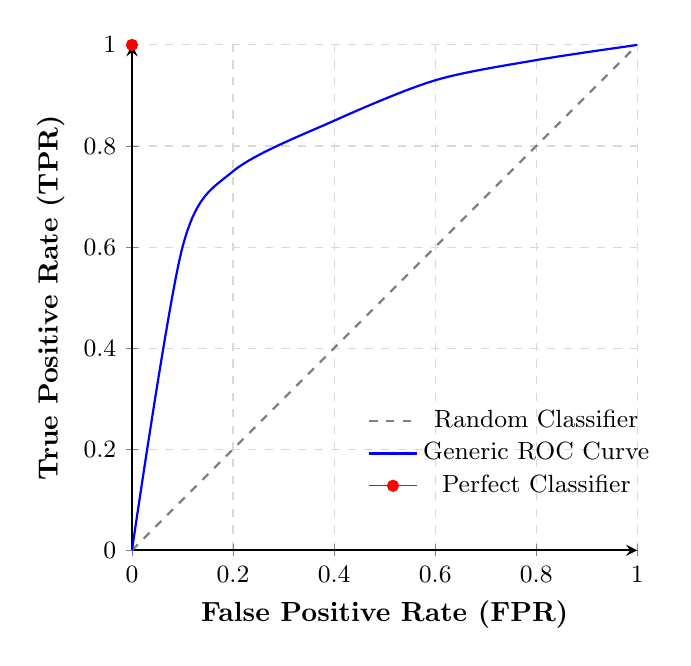
\begin{tikzpicture}
    \begin{axis}[
      width=8cm, height=8cm,
      grid=both, % Adds grid
      grid style={dashed, gray!30},
      xlabel={False Positive Rate (FPR)},
      ylabel={True Positive Rate (TPR)},
      xmin=0, xmax=1, % Limits for x-axis (FPR)
      ymin=0, ymax=1, % Limits for y-axis (TPR)
      axis lines=left,
      axis line style={thick},
      label style={font=\bfseries},
      tick label style={font=\small},
      xtick={0,0.2,0.4,0.6,0.8,1}, % X-axis ticks
      ytick={0,0.2,0.4,0.6,0.8,1}, % Y-axis ticks
      legend style={at={(0.45,0.3)},anchor=north west,draw=none,fill=none, font=\small}
    ]
  
    % Plotting the random classifier (diagonal)
    \addplot[domain=0:1, thick, dashed, gray] {x};
    \addlegendentry{Random Classifier}
  
    % Plotting the ROC curve for a typical classifier
    \addplot[thick, smooth, blue] coordinates {
      (0,0) (0.1,0.6) (0.2,0.75) (0.4,0.85) (0.6,0.93) (0.8,0.97) (1,1)
    };
    \addlegendentry{Generic ROC Curve}
  
    % Highlighting the perfect point (0,1)
    \addplot[mark=*, mark size=2pt, color=red] coordinates {(0,1)};
    \node[above right] at (axis cs: 0,1) {};
    \addlegendentry{Perfect Classifier}
  
    \end{axis}
  \end{tikzpicture} 
    \caption[Illustrazione di una generica curva ROC.]{Illustrazione di una generica curva ROC.}\label{fig:ROC-curve} 
\end{figure}
% 
Come si può ossevrare nella Figura\,\ref{fig:ROC-curve}, vengono rappresentate tre casistiche. La linea retta, tratteggiata, rappresenta un modello casuale, ovvero che classifica i dati senza criterio. La linea blu rappresenta un modello generico. All'inizio della curva si può osservare che il \acs{FPR} cresce lentamente rispetto al \acs{TPR}, indicando che il modello riesce ad identificare molti veri positivi senza classificare molti falsi positivi. In questo caso, la soglia è molto elevata, poiché è necessario che un elemento abbia un'alta probabilità di apparteneza alla classe affinché venga classificato nella categoria positiva. Man mano che la soglia diminuisce si osserva che sia il \acs{TPR} che il \acs{FPR} del modello salgono in quanto molti più elementi vengono classificati nella categoria positiva, anche se la classe reale è quella negativa. Il punto rosso rappresenta il modello ideale, che ha il massimo valore di \acs{TPR} (ovvero 1) e il minimo valore di \acs{FPR} (cioè 0).

Per semplificare la lettura della curva \acs{ROC}, spesso viene utilizzato il valore dell'area sotto la curva, chiamato \acs{AUC}, \textit{Area Under the Curve} — o anche \acs{AUROC}, \textit{Area Under the \acs{ROC} Curve}.
% 
\begin{figure}[!b]
    \centering
    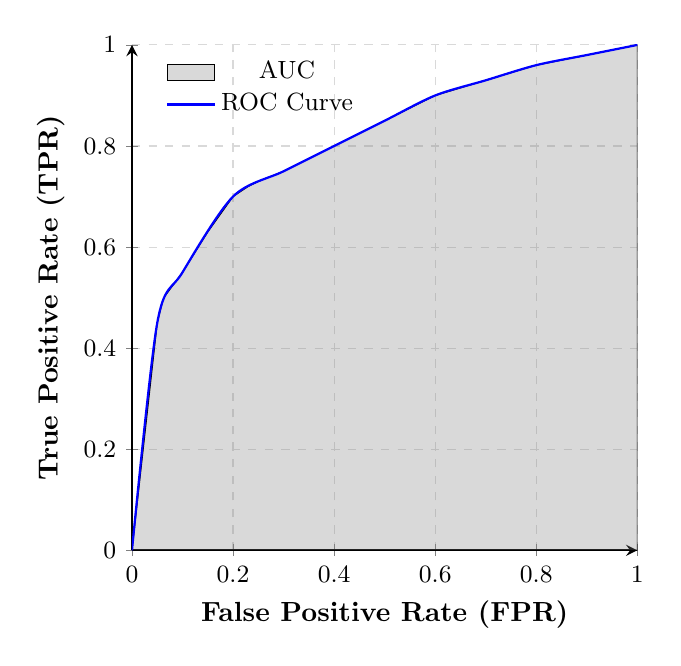
\begin{tikzpicture}
    \begin{axis}[
      width=8cm, height=8cm,
      grid=both, % Adds grid
      grid style={dashed, gray!30},
      xlabel={False Positive Rate (FPR)},
      ylabel={True Positive Rate (TPR)},
      xmin=0, xmax=1, % Limits for x-axis (FPR)
      ymin=0, ymax=1, % Limits for y-axis (TPR)
      axis lines=left,
      axis line style={thick},
      label style={font=\bfseries},
      tick label style={font=\small},
      xtick={0,0.2,0.4,0.6,0.8,1}, % X-axis ticks
      ytick={0,0.2,0.4,0.6,0.8,1}, % Y-axis ticks
      legend style={at={(0.05,0.99)},anchor=north west,draw=none,fill=none, font=\small}
    ]
  
    % Shaded area under the ROC curve (AUC) with improved precision
    \addplot[
      domain=0:1,
      samples=200,
      fill=gray,
      fill opacity=0.3,
      area legend
    ]
    coordinates {
      (0,0) (0.05,0.45) (0.055,0.47) (0.06,0.49) (0.063,0.5) (0.1,0.55) (0.15,0.63) (0.2,0.7) (0.23,0.72) (0.25,0.73) (0.3,0.75) (0.4,0.8) (0.5,0.85) (0.6,0.9) (0.7,0.93) (0.8,0.96) (0.9,0.98) (1,1) (1,0) (0,0)
    };
    \addlegendentry{AUC}
  
    % Plotting the ROC curve for a typical classifier with a thicker line
    \addplot[thick, smooth, blue] coordinates {
      (0,0) (0.05,0.45) (0.1,0.55) (0.2,0.7) (0.3,0.75) (0.4,0.8) (0.5,0.85) (0.6,0.9) (0.7,0.93) (0.8,0.96) (0.9,0.98) (1,1)
    };
    \addlegendentry{ROC Curve}
  
    \end{axis}
  \end{tikzpicture} 
    \caption[Area sottesa alla curva \acs{ROC}.]{Area sottesa alla curva \acs{ROC}. Questo valore viene comunemente utilizzato per paragonare diversi modelli.}\label{fig:AUC-value} 
\end{figure}
% 
Questo valore aiuta notevolmente a riassumere le capactà predittive dell'algoritmo in un solo numero (Figura\,\ref{fig:AUC-value}). È stato dimostrato che questo valore fornisce valori più significativi rispetto ad altre metriche, tra cui l'accuratezza\footnote{L'accuratezza di un modello è data dal rapporto tra le predizioni corrette del modello (TP e TN) con l'intero dataset.}\,\cite{huang2005using}. Inoltre questo valore è anche più comodo per paragonare le performance di due modelli, piuttsto che comparare le curve \acs{ROC}: proprio per questo motivo è ad oggi una tra le metriche utilizzate per la valutazione di modelli di \acs{DL}.



\section{Reti neurali convoluzionali}
% 
Le reti neurali convoluzionali (\acs{CNN}) sono state introdotte per la prima volta nel 1998, con la pubblicazione dell'articolo ``Gradient-based learning applied to document recognition''\,\cite{lecun1998gradient} il quale descrive una rete artificiale, chiamata \textit{LeNet-5}, il obiettivo era quello di identificare documenti scritti a mano. Questo articolo getta le basi per la progettazione di una rete convoluzionale\,\cite{aggarwal2018neural}.

Una rete convoluzionale è una rete neurale feedforward che contiene dei particolari livelli, volti a ridurre il numero di pesi della rete. Tre sono i layer fondamentali che caratterizzano una \acs{CNN}: \textit{convolution layer}, \textit{padding layer} e \textit{\acs{ReLU} layer}. Queste reti, sono organizzate in modo tale da riconoscere le caratteristiche spaziali di un immagine. Per questo motivo, generalmente, si rappresenta l'input layer come una matrice bidimensionale\footnote{Ipotizzando, per semplicità, che l'immagine sia in scala di grigi.} di pixel: in questo modo viene anche facilitata la comprensione delle operazioni che processano l'input.

\subsection{Livello convoluzionale}
% 
Nelle reti neurali convoluzionali, i parametri sono raggruppati in unità bidimensionali chiamati filtri o \textit{kernel}. Questi sono delle matrici, generalmente quadrate, dimensionalmente minori rispetto alla grandezza dell'input. Tali unità rendono possibile l'operazione di convoluzione con il livello precedente. Come mostrato nella Figura\,\ref{fig:convolution-operation}, la convoluzione fa scorrere il filtro $K$ sulla matrice $M$ e, per ogni spostamento, calcola il prodotto scalare tra il kernel e i valori di $M$ selezionati in quell'istante.
% 
\begin{figure}[!b]
    \centering
    \input{assets/TikZ/convolution-operation.tex}
    \caption[L'operazione di convoluzione in una matrice bidimensionale.]{L'operazione di convoluzione in una matrice bidimensionale (adattata da\,\cite{janosh_convolution}).}\label{fig:convolution-operation}
\end{figure}
% 
Si osserva che il numero di valori risultanti da questa operazione è esattamente il numero di neuroni che sono presenti nel livello successivo. Questo valore si può calcolare in maniera semplice, conoscendo le dimensioni della matrice iniziale e del kernel. Fornite il numero di colonne della matrice, ovvero la sua larghezza $w$, e il numero di righe, ovvero la sua altezza $h$, allora, applicando una convoluzione con un filtro $n \times n$ le dimensioni al livello $\ell + 1$ valgono:
% 
\begin{gather*}
    w^{(\ell + 1)} = w^{(\ell)} - n + 1
    \hspace{60px}
    h^{(\ell + 1)} = h^{(\ell)} - n + 1
\end{gather*}
% 
Osservando la Figura\,\ref{fig:convolution-operation} si nota che la matrice $M$ di dimensione $7\times 7$ diventa una matrice $5 \times 5$ quando applicata una convoluzione con un filtro di dimensione $3\times 3$. Si specifica inoltre che tra un livello e quello successivo, non si esegue una sola operazione di convoluzione, bensì vengono compiute più convoluzioni, ciascuna con un filtro diverso (anche se della stessa dimensione). Di conseguenza, il risultato di queste operazioni sarà un numero di matrici $d$, che corrispondono al numero di filtri con cui è stata attuata la convoluzione sul livello precedente. L'applicazione di più filtri sullo stesso livello rende possibile riconoscere pattern particolari: per esempio è possibile utilizzare un insieme di filtri per riconoscere una sagoma all'interno di un'immagine. In questo modo, in una \acs{CNN} è possibile avere diversi livelli convoluzionali tali per cui ciascuno riconosce un particolare pattern dall'immagine iniziale sempre più complesso. Avere più livelli convoluzionali che processano l'immagine fa si che l'ultimo livello convoluzionale esamini porzioni più ampie dell'immagine, riconoscendo caratteristiche e strutture più articolate\,\cite{aggarwal2018neural, wu2017introduction}.
% 
\begin{figure}[!t]
    \centering
    \input{assets/TikZ/convolutional-neural-network.tex}
    \caption[Rappresentazione di una rete neurale convoluzionale.]{Rappresentazione di una rete neurale convoluzionale. Si fa notare la presenza di più livelli convoluzionali che permettono l'estrazione di pattern progressivamente più complessi (adattata da\,\cite{izaak2022neural}).}\label{fig:convolutional-neural-network}
\end{figure}

Come notato in precedenza, dopo ogni livello di convoluzione, la dimensione dell'immagine è ridotta in proporzione alla grandezza del filtro. In genere, la riduzione dimensionale comporta perdita di informazioni e va evitata. Per questo motivo, prima di fare l'operazione di convoluzione, si effettua il padding. Attraverso questa operazione, si aggiungono una serie di ``0''\footnote{Si è scelto il valore zero proprio perché non ha effetto e non distorce il risultato numerico della convoluzione.} lungo i bordi dell'immagine in modo tale che, una volta processata, rimanga della stessa dimensione. In ogni bordo dell'immagine vengono aggiungi esattamente $(n - 1) / 2$ pixel, dove $n$ è la dimensione del filtro. 
% 
\begin{figure}[!t]
    \centering
    \begin{tikzpicture}[
    2d-arr/.style={matrix of nodes, row sep=-\pgflinewidth, column sep=-\pgflinewidth, nodes={draw}},
    pad/.style={fill=gray!30} % style for padding (light gray)
  ]
  
  % Enlarged matrix with padding (9x9 matrix)
  \matrix (mtr) [2d-arr] {
  |[pad]| 0 & |[pad]| 0 & |[pad]| 0 & |[pad]| 0 & |[fill=yellow!30]| 0 & |[fill=yellow!30]| 0 & |[fill=yellow!30]| 0 & |[pad]| 0 & |[pad]| 0\\
  |[pad]| 0 & 0 & 1 & 1 & |[fill=yellow!30]| 1 & |[fill=yellow!30]| 0 & |[fill=yellow!30]| 0 & 0 & |[pad]| 0\\
  |[pad]| 0 & 0 & 0 & 1 & |[fill=yellow!30]| 1 & |[fill=yellow!30]| 1 & |[fill=yellow!30]| 0 & 0 & |[pad]| 0\\
  |[pad]| 0 & 0 & 0 & 0 & 1 & 1 & 1 & 0 & |[pad]| 0\\
  |[pad]| 0 & 0 & 0 & 0 & 1 & 1 & 0 & 0 & |[pad]| 0\\
  |[pad]| 0 & 0 & 0 & 1 & 1 & 0 & 0 & 0 & |[pad]| 0\\
  |[pad]| 0 & 0 & 1 & 1 & 0 & 0 & 0 & 0 & |[pad]| 0\\
  |[pad]| 0 & 1 & 1 & 0 & 0 & 0 & 0 & 0 & |[pad]| 0\\
  |[pad]| 0 & |[pad]| 0 & |[pad]| 0 & |[pad]| 0 & |[pad]| 0 & |[pad]| 0 & |[pad]| 0 & |[pad]| 0 & |[pad]| 0\\
  };
  
  \node[below=of mtr-8-5] {$\mathbf{M}_{padded}$};
  
  \node[right=0.2em of mtr] (str) {$*$};
  
  % Convolution kernel (same 3x3 matrix)
  \matrix (K) [2d-arr, right=0.2em of str, nodes={draw, fill=blue!15}] {
    1 & 0 & 1 \\
    0 & 1 & 0 \\
    1 & 0 & 1 \\
  };
  \node[below=of K-2-2] {$\mathbf K$};
  
  \node[right=0.2em of K] (eq) {$=$};
  
  % Resulting matrix after convolution (7x7 matrix)
  \matrix (ret) [2d-arr, right=0.2em of eq] {
    0 & 2 & 2 & 3 & |[fill=green!30]| 1 & 1 & 0 \\
    1 & 1 & 4 & 3 & 4 & 1 & 1 \\
    0 & 1 & 2 & 4 & 3 & 3 & 0 \\
    0 & 1 & 2 & 3 & 4 & 1 & 1 \\
    1 & 1 & 3 & 3 & 1 & 1 & 0 \\
    1 & 3 & 3 & 1 & 1 & 0 & 0 \\
    2 & 2 & 1 & 1 & 0 & 0 & 0 \\
  };
  \node[below=of ret-6-4] {$\mathbf{M}_{padded} * \mathbf{K}$};
  
  % Connection lines showing how convolution is applied
  \draw[dashed, blue!60] (mtr-1-7.north east) -- (K-1-1.north west);
  \draw[dashed, blue!60] (mtr-3-7.south east) -- (K-3-1.south west);
  
  \draw[dashed, green!60] (K-1-3.north east) -- (ret-1-5.north west);
  \draw[dashed, green!60] (K-3-3.south east) -- (ret-1-5.south west);
  
  % Multiplication annotations for elements inside yellow box
  \foreach \i in {1,2,3} {
      \foreach \j in {5,6,7} {
          \node[font=\tiny, scale=0.6, shift={(-1.2ex,-2ex)}] at (mtr-\i-\j) {$\times \pgfmathparse{int(mod(\i+\j,2))}\pgfmathresult$};
      }
  }
  
  \end{tikzpicture}
  
    \caption[Padding di una matrice che precede la convoluzione.]{Padding di una matrice che precede la convoluzione. In questo modo, la dimensione della matrice rimane invariata dopo la convoluzione (adattata da\,\cite{janosh_convolution}).}\label{fig:padding}
\end{figure}
% 
La Figura\,\ref{fig:padding} illustra l'operazione di convoluzione presentata nella Figura\,\ref{fig:convolution-operation} con la differnza che la matrice iniziale ha subito l'operazione di padding. Notando le due figure si osserva che nel primo caso il risultato della convoluzione ha ridotto la dimensione iniziale delle matrice mentre nel secondo caso, attraverso il padding, la dimensione rimane invariata grazie ai valori inseriti lungo i bordi della matrice\,\cite{aggarwal2018neural}.

\subsection{Livello \acs{ReLU}}

In genere, ogni livello convoluzionale è seguito da un \acs{ReLU} layer (\textit{Rectified Linear Unit}). Questo livello sostituisce la funzione di attivazione sigmoidale con una funzione detta rettificatrice, definita come segue:
% 
\begin{gather*}
    \text{ReLU}(x) = \max{\left(0,\,x\right)} = 
    \begin{cases}
        x \hspace{20px} \text{se } v>0\\
        0 \hspace{20px} \text{se } v\leq0
    \end{cases}
\end{gather*}
% 
\noindent Si osserva che, a differenza del livello convoluzionale, questo livello non modifica la dimensione della matrice in quanto mappa direttamente i dati presenti senza alterarne la struttura. La funzione di attivazione \acs{ReLU}, rappresentata nella Figura\,\ref{fig:relu-function}, è stata introdotta recentemente nelle reti neurali in quanto fornisce diversi vantaggi rispetto alle funzioni sigmoidali, soprattutto per quanto riguarda la velocità dell'allenamento\footnote{Questo perché la derivata di una retta è molto più semplice rispetto alla derivata della funzione sigmoide.}\,\cite{aggarwal2018neural}.
% 
\begin{figure}[!t]
    \centering
    \begin{tikzpicture}
    \begin{axis}[
        axis lines = middle,
        xlabel = $x$,
        ylabel = {ReLU$(x)$},
        samples = 100,
        domain = -2:2,
        ymin = -0.5, ymax = 2,
        xmin = -2, xmax = 2,
        width=10cm,
        height=7cm,
        xtick={-2,-1,0,1,2},
        ytick={0,1,2},
        enlargelimits
      ]
      % ReLU function definition
      \addplot[color=red, thick] {max(0,x)}; 
    \end{axis}
  \end{tikzpicture}
  
    \caption[Grafico della funzione rettificatrice \textsl{ReLU}$(x)$.]{Grafico della funzione rettificatrice \textbf{ReLU}$(x)$.}\label{fig:relu-function}
\end{figure}

\subsection{Livello di pooling}

Dopo aver processato le infomazioni mediante la convoluzione, al fine di alleggerire il carico computazionale, si cerca di concentrare le informazioni estratte attraverso il \textit{pooling}. Il tipo di pooling più comune nelle \acs{NN} è il \textit{max-pooling}. Questa operazione, in maniera simile ad un filtro, scorre lungo la matrice ed estrae dalla zona selezionata il valore massimo (Figura\,\ref{fig:max-pooling-operation}).
% 
\begin{figure}[!b]
    \centering
    \begin{tikzpicture}[
    2d-arr/.style={matrix of nodes, row sep=-\pgflinewidth, column sep=-\pgflinewidth, nodes={draw}}
  ]
  
  \matrix (mtr) [2d-arr] {
    3 & 7 & |[fill=orange!20]| 4 & |[fill=orange!20]| 1 & |[fill=orange!20]| 6 & 0 & 0\\
    2 & 9 & |[fill=orange!20]| 1 & |[fill=orange!30]| 8 & |[fill=orange!20]| 5 & 0 & 0\\
    0 & 4 & |[fill=orange!20]| 0 & |[fill=orange!20]| 6 & |[fill=orange!20]| 7 & 3 & 0\\
    5 & 1 & 0 & 2 & 8 & 0 & 0\\
    0 & 0 & 3 & 9 & 0 & 0 & 4\\
    1 & 6 & 7 & 0 & 2 & 0 & 0\\
    8 & 0 & 0 & 0 & 1 & 0 & 0\\
  };
  
  \node[below=of mtr-6-4] {$\mathbf M$};

  \matrix (ret) [2d-arr, right=6em of mtr] {
    9 & 9 & |[fill=red!20]| 8 & 8 & 7 \\
    9 & 9 & 8 & 8 & 8 \\
    5 & 9 & 9 & 9 & 8 \\
    7 & 9 & 9 & 9 & 8 \\
    8 & 9 & 9 & 9 & 4 \\
  };

  \node[below=of ret-5-3] {$\mathbf{M}_{pooled}$};

  
  \draw[dashed, orange!60!red] (mtr-1-5.north east) -- (ret-1-3.north west);
  \draw[dashed, orange!60!red] (mtr-3-5.south east) -- (ret-1-3.south west);
  
  \end{tikzpicture}

    \caption[Operazione di max-pooling in una matrice.]{Operazione di max-pooling in una matrice. Questa operazione permette di estrarre le caratterestiche dominanti dopo la convoluzione (adattata da\,\cite{janosh_convolution}).}\label{fig:max-pooling-operation}
\end{figure}
% 
L'idea dietro al max-pooling è quella di tenere le caratteristiche prevalenti dalla matrice fornita, in modo da ridurre l'informazione per rendere la fase di allenamento meno onerosa. Al max-pooling si aggiunge anche il \textit{avg-pooling} che si occupa di calcolare la media dei pixel presenti nella porzione selezionata, estraendo quindi la ``proprietà media'' anzichè quella prevalente\,\cite{aggarwal2018neural, o2015introduction}.

Infine, come in tutte le reti neurali, in una \acs{CNN} sono presenti i \textit{fully-connected layers}. Questi livelli, che sono presenti solo dopo i livelli convoluzionali (come mostrato nella Figura\,\ref{fig:convolutional-neural-network}), hanno la stessa funzione di una classica feedforward \acs{NN}: effettuare una serie di calcoli che permette di predire correttamente la risposta, in funzione dell'input fornito\,\cite{aggarwal2018neural, o2015introduction}.

\subsection{Applicazioni}

Anche se fino ad ora le \acs{CNN} sono state descritte come tool che processa solo immagine, il loro utilizzo è in realtà molto più vasto. Tra le loro numerose applicazioni, vengono citate il \textit{Natural Language Processing} (\acs{NLP}) — disciplina che si occupa di processare il linguaggio naturale, attraverso il riconoscimento vocale e la classificazione del testo — e \textit{Computer Vision} — che comprende il riconoscimento visivo, la \textit{scene labelling} e il riconoscimento di oggetti e azioni umane\,\cite{shamsaldin2019study, li2021survey, bhatt2021cnn}.

Oltre a quanto menzionato, le reti neurali convoluzionali, sono largamente utilizzate nel campo della bioinformatica. Più precisamente, le \acs{CNN} $1$-dimensionali\footnote{Ovvero che l'input si estende in una dimensione, proprio come una sequenza.} analizzando sequenze di \acs{DNA} ed \acs{RNA}, apprendendo pattern — che in bioinformatica vengono anche chiamati \textit{motif} — sequenziali man mano più complessi attraverso i diversi layer convoluzionali. In questo modo è possibile approfondire i problemi che riguardano gli elementi regolatori dell'espressione genica, tra cui le varianti non codificanti\,\cite{min2017deep}.






% Invarianti, notazioni
\begin{comment}
    Per non diventare matti la notazione è l'opposta di quella sul file di Machine Learnign.
    - ci sono esattamente N feature in un vettore di input, di conseguenza il vettore di pesi è di lunghezza N
    - ci sono esattamente M vettori di input nel dataset, di conseguenza la lunghezza della label è M
    - Il dataset D è composta da j colonne ed i righe
    - Ciascuna riga j rappresenta un elemento del dataset
    - Ciascuna colonna i rappresente un feature del dataset
    
    Di conseguneza D_j indica il vettore j-esimo composto esattamente da N componenti. La label y_j indica il vero valore dell'input processato
\end{comment}

% https://www.researchgate.net/profile/Shashi-Sathyanarayana/publication/266396438_A_Gentle_Introduction_to_Backpropagation/links/577d124808aeaa6988aba0bc/A-Gentle-Introduction-to-Backpropagation.pdf

% https://d1wqtxts1xzle7.cloudfront.net/51924347/NeuralNetworks-libre.pdf?1487958246=&response-content-disposition=inline%3B+filename%3DBack_Propagation_Algorithm.pdf&Expires=1725992239&Signature=J-LZ7rIZD5T6Nb9jar55PvgTCF3pDd0H8dGNJVU3ijf1bFEoiAX2yF9fkroyCTvPGm0oAhX8SUhRLSZ26bEVOC08ZV9wUPb8HekE0~cj836hKUsc60DVhhXQ3TjlPE91VTwe0kMkDuimtxQuf8LVgJhSF5zc~sAFzSOmHwPfbiqBTxNoSFRY8xkMRRNoTMWS1GZmoOr83rB3VkzKA6QncuQ85ogs4IHeInFT2nnqBNUbvUGOEyhDUbECy39bE57G1CkhMRIXiT-CZLPJxY1gu2dYjr7~gerF49Lay6w1yNJ5kdgqrMpy5TI8suaIwC0NQZ1obOrERVpDKrJ3Y~Lrhg__&Key-Pair-Id=APKAJLOHF5GGSLRBV4ZA
